\documentclass[a4paper,11pt]{ltjsarticle}
% 数式
\usepackage{amsmath,amsfonts}
\usepackage{bm}
% 画像
\usepackage{graphicx}
\usepackage{circuitikz}
\usepackage{amsmath,amssymb}
\usepackage{siunitx}
\usepackage{float}
\usepackage{tikz}
\usepackage{askmaps}
\usepackage{multirow}
\usepackage{bigstrut}
\usepackage{slashbox}
\usepackage{rotating}
\usepackage{listings}
% 数式
\usepackage{physics}
\usepackage{mathtools}
% 画像
\usepackage{subcaption}
% 表
\usepackage{makecell}
% その他
\usepackage{url}
\usepackage{ascmac}
\usepackage{cases}
\usepackage{here}
\usepackage{upgreek}
% 日本語対応
\usepackage{luatexja}
\usepackage{luatexja-fontspec}

\AtBeginDocument{\RenewCommandCopy\qty\SI}


\definecolor{commentgreen}{RGB}{0,200,0}
\definecolor{eminence}{RGB}{120,80,250}
\definecolor{weborange}{RGB}{255,165,0}
\definecolor{frenchplum}{RGB}{10,150,200}
\definecolor{commentgreen}{RGB}{0,200,0}
\definecolor{eminence}{RGB}{120,80,250}
\definecolor{weborange}{RGB}{255,165,0}
\definecolor{frenchplum}{RGB}{10,150,200}

\lstset{
        language = {C},
        basicstyle = \ttfamily\small,
        keywordstyle=\color{eminence}\ttfamily\bfseries,
        commentstyle=\color{commentgreen}\textit,
    identifierstyle=\color{black}\ttfamily,
        xleftmargin=.35in,
        frame=lines,
    showstringspaces=false,
        numbers=left,
        stepnumber = 1,
        breaklines=true,
        numberstyle = \ttfamily\normalsize,
    tabsize=4,  
        emph={int, int8_t, int16_t, int32_t, int64_t, uint8_t, uint16_t, uint32_t, uint64_t, char, double, float, unsigned, void, bool},
        emphstyle={\color{blue}}, 
        morekeywords={>, <, ., ;, +, -, *, /, !, =, ~},
        breakindent = 10pt, 
        framexleftmargin=10mm, 
        columns=fixed,
        basewidth=0.5em,
        }

% 特定のスタイル設定
\lstdefinestyle{customtxt}{
  basicstyle=\ttfamily\footnotesize,
  backgroundcolor=\color{lightgray},
  frame=single,
  breaklines=true,
  columns=fullflexible,
  showspaces=false,
  showstringspaces=false,
  showtabs=false,
  tabsize=4,
}

\newcommand{\fig}[4]{
    \begin{figure}[htbp]
      \centering
      \includegraphics{./image/#1}
      \caption{#2}
      \label{fig:#3}
    \end{figure}
  }
\begin{document}
$A=\overline{IN_2}\cdot\overline{IN_1} \cdot IN_0 \cdot EN + IN_2 \cdot \overline{IN_1} \cdot \overline{IN_0} \cdot EN + \overline{EN}$
\section{目的}
本実験では，簡単な組み合わせ回路をHDLで設計し，シュミレーションを行い，
FPGAについてHDLの書き方と内部の動作を理解することを目的とする．
また，FPGAボードにおいて実際に動作させることで，ブロック図からHDL，そして実機へのプログラムの一連の流れを学ぶことを目的とする．
\section{原理}
本実験で使用するGPGA，HDL，Verilogについて説明する．
\subsection{FPGA}
FPGA(Field Programmable Gate Array)は，ユーザが設計した論理回路を実装できるLSIである．
FPGAは，AND回路などの基本的な論理素子を内部に持っており，それをユーザーのプログラムによって内部で接続させることにより
，様々な論理回路を実現できるものである．集積回路の設計において，回路をプログラムから変更できる点により
小規模開発に適しているといえる．
\subsection{HDL}
HDL(Hardware Description Language)は，ハードウェアを記述するための言語である．
HDLを用いることにより，論理回路の設計をテキストベースで行うことができる．
HDLには，VerilogやVHDLなどがある．
\subsection{Verilog}
Verilogは，HDLの一種であり，C言語に似た構文を持つ．
Verilogでは，モジュールという単位で回路を記述する．モジュールには，入力ポート，出力ポート，内部信号などがあり，
モジュールからモジュールを呼び出して回路を組み合わせることが出来る．
またモジュール内では，論理演算や条件分岐，繰り返しなどの構文を用いて回路を記述することができる．
\section{実験環境}
表\ref{tab:zikken}に使用するソフトウェアとハードウェアについての実験環境を示す．
\begin{table}[H]
  \centering
  \caption{実験環境}
  \label{tab:zikken}
  \begin{tabular}{|c|c|}
    \hline
    項目             & 内容                                   \\
    \hline
    FPGAボード        & Gowin社製 GW1NR-9                      \\
    \hline
    開発ソフトウェア       & Gowin\_V1.9.11.03 Education (64-bit) \\
    \hline
    シミュレーションソフトウェア & iverilog                             \\
    \hline
  \end{tabular}
\end{table}
\section{実験方法}
本実験は課題に沿って実験を行っていく．課題に沿った実験方法を本章で説明する．
\subsection{ブロック図}
全加算器/全減算機の組み合わせ回路を本実験で作成を行う．そのため入力から出力までの回路図をブロック図として作成を行う．
\subsection{HDLの作成}
ブロック図をもとにHDLを作成する．本実験ではVerilogを用いてHDLを作成する．
\subsection{シミュレーション}
作成したHDLが正しく動作するかをテストベンチを作成し，シミュレーションを行い確認する．
\subsection{FPGAへの書き込み}
シミュレーションで正しく動作することが確認できたら，FPGAボードに書き込みを行い，シュミレーションと同じ動きをするか確認する．
\subsection{動作確認}
FPGAボードに書き込みを行った後，実際に動作確認を行う．
\section{結果}
実験方法を参照し，各課題に沿って実験を行った．
\subsection{ブロック図}
図\ref{fig:block}に全加算器/全減算機の組み合わせ回路のブロック図を示す．
\begin{figure}[H]
  \centering
  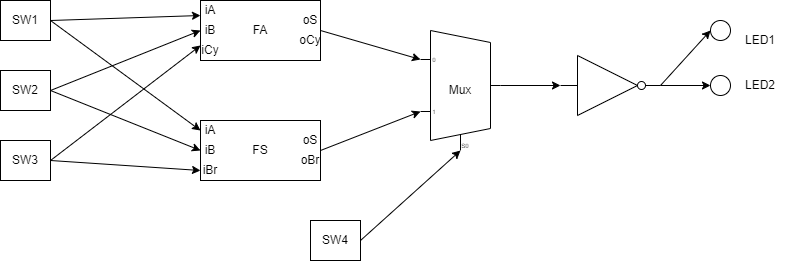
\includegraphics[width=0.8\linewidth]{./image/block.drawio.png}
  \caption{全加算器/全減算機の組み合わせ回路のブロック図}
  \label{fig:block}
\end{figure}
\subsection{HDLの作成}
作成したverilogコードを順に示す．
半加算器のVerilogコードをリスト\ref{lst:half_adder}に示す．
全加算器のVerilogコードをリスト\ref{lst:full_adder}に示す．
半減算器のVerilogコードをリスト\ref{lst:half_subtractor}に示す．
全減算器のVerilogコードをリスト\ref{lst:full_subtractor}に示す．
全加算器/全減算機の組み合わせ回路のVerilogコードをリスト\ref{lst:full_adder_subtractor}に
示す．
\begin{lstlisting}[caption=半加算器のVerilogコード,label=lst:half_adder]
module HalfAdder(iA, iB, oS, oCy);
	input iA;
	input iB;
	output oS;
	output oCy;

	assign oS = (iA ^ iB);
	assign oCy = (iA & iB);
endmodule
\end{lstlisting}
\begin{lstlisting}[caption=全加算器のVerilogコード,label=lst:full_adder]
  module FullAdder(iA, iB, iCy, oS, oCy);
	input iA;
	input iB;
	input iCy;
	output oS;
	output oCy;

	wire HA1_S;
	wire HA1_C;
	wire HA2_C;

	HalfAdder HA1 (
		.iA(iA),
		.iB(iB),
		.oS(HA1_S),
		.oCy(HA1_C)
	);
	HalfAdder HA2 (
		.iA(HA1_S),
		.iB(iCy),
		.oS(oS),
		.oCy(HA2_C)
	);
	assign oCy = HA1_C | HA2_C;
endmodule
\end{lstlisting}
\begin{lstlisting}[caption=半減算器のVerilogコード,label=lst:half_subtractor]
module HalfSub(iA, iB, oS, oCy);
	input iA;
	input iB;
	output oS;
	output oCy;

	assign oS = (iA ^ iB);
	assign oCy = (~iA & iB);
endmodule
\end{lstlisting}
\begin{lstlisting}[caption=全減算器のVerilogコード,label=lst:full_subtractor]
module FullSub(iA, iB, iCy, oS, oCy);
	input iA;
	input iB;
	input iCy;
	output oS;
	output oCy;

	wire HA1_S;
	wire HA1_C;
	wire HA2_C;

	HalfSub HS1 (
		.iA(iA),
		.iB(iB),
		.oS(HA1_S),
		.oCy(HA1_C)
	);
	HalfSub HS2 (
		.iA(HA1_S),
		.iB(iCy),
		.oS(oS),
		.oCy(HA2_C)
	);
	assign oCy = HA1_C | HA2_C;
endmodule
\end{lstlisting}
\begin{lstlisting}[caption=全加算器/全減算機の組み合わせ回路のVerilogコード,label=lst:full_adder_subtractor]
module MAIN(AS_sel,iA, iB, iCy, oS, oCy);
    input AS_sel;
	input iA;
	input iB;
	input iCy;
	output oS;
	output oCy;

	wire [1:0] FA_res;
	wire [1:0] FS_res;

	FullAdder FA (
		.iA(iA),
		.iB(iB),
        .iCy(iCy),
		.oS(FA_res[0]),
		.oCy(FA_res[1])
	);
	FullSub FS (
		.iA(iA),
		.iB(iB),
        .iCy(iCy),
		.oS(FS_res[0]),
		.oCy(FS_res[1])
	);
    function [1:0] SelF;
        input [1:0] iA;
        input [1:0] iB;
        input iSw;
        begin
            case(iSw)
                2'b0: SelF =  iA;
                2'b1: SelF =  iB;
            default: SelF=2'bXX;
            endcase
        end
    endfunction
    assign {oS,oCy} = ~SelF(FA_res, FS_res, AS_sel);
endmodule
\end{lstlisting}
\subsection{シミュレーション}
作成したHDLが正しく動作するかをテストベンチを作成し，シミュレーションを行い確認した．
全加算器/全減算機の組み合わせ回路のテストベンチコードをリスト\ref{lst:testbench}に示す．
\begin{lstlisting}[caption=全加算器/全減算機の組み合わせ回路のテストベンコード,label=lst:testbench]
module MAINTEST;

reg a, b,c,d;
wire e,f;

MAIN and_instance(d, c, b,a,e,f);

initial begin
        $dumpfile("main.vcd");
        $dumpvars(1, MAINTEST);
        
        a = 0; b = 0;c = 0;d = 0;
        #10 a = 1;
        #10 a = 0; b = 1;
        #10 a = 1;
        #10 a = 0; b = 0;c = 1;
        #10 a = 1;
        #10 a = 0; b = 1;
        #10 a = 1;
        #10 a = 0; b = 0;c = 0;d = 1;
        #10 a = 1;
        #10 a = 0; b = 1;
        #10 a = 1;
        #10 a = 0; b = 0;c = 1;
        #10 a = 1;
        #10 a = 0; b = 1;
        #10 a = 1;
        #10 $finish;
end

endmodule
\end{lstlisting}
シミュレーション結果を図\ref{fig:sim}に示す．
\begin{figure}[H]
  \centering
  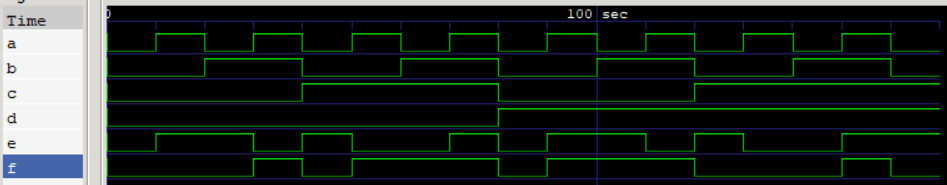
\includegraphics[width=0.8\linewidth]{./image/sim.png}
  \caption{シミュレーション結果}
  \label{fig:sim}
\end{figure}
\subsection{FPGAへの書き込み}
シミュレーションで正しく動作することが確認できたため，FPGAボードに書き込みを行った．
また，設定を行ったピン番号をリスト\ref{lst:pin}に示し，各信号との対応表を表\ref{tab:pin}に示す．
そして，FPGAボードではLEDが反転しているため，確認のしやすさのためにブロック図においてマルチプレクサとLEDの間に反転回路を挿入している．
\begin{lstlisting}[caption=FPGAピン設定コード,label=lst:pin]
//Copyright (C)2014-2025 Gowin Semiconductor Corporation.
//All rights reserved. 
//File Title: Physical Constraints file
//Tool Version: V1.9.11.03 Education
//Part Number: GW1NR-LV9QN88PC6/I5
//Device: GW1NR-9
//Device Version: C
//Created Time: Tue 12 09 00:44:23 2025

IO_LOC "oCy" 10;
IO_PORT "oCy" IO_TYPE=LVCMOS18 PULL_MODE=NONE DRIVE=8 BANK_VCCIO=1.8;
IO_LOC "oS" 11;
IO_PORT "oS" IO_TYPE=LVCMOS18 PULL_MODE=NONE DRIVE=8 BANK_VCCIO=1.8;
IO_LOC "iCy" 57;
IO_PORT "iCy" IO_TYPE=LVCMOS18 PULL_MODE=NONE BANK_VCCIO=1.8;
IO_LOC "iB" 68;
IO_PORT "iB" IO_TYPE=LVCMOS18 PULL_MODE=NONE BANK_VCCIO=1.8;
IO_LOC "iA" 69;
IO_PORT "iA" IO_TYPE=LVCMOS18 PULL_MODE=NONE BANK_VCCIO=1.8;
IO_LOC "AS_sel" 56;
IO_PORT "AS_sel" IO_TYPE=LVCMOS18 PULL_MODE=NONE BANK_VCCIO=1.8;
\end{lstlisting}
\begin{table}[H]
  \centering
  \caption{各信号との対応表}
  \label{tab:pin}
  \begin{tabular}{|c|c|c|c|}
    \hline
    信号名     & ピン番号 IOTYPE & PULL MODE \\
    \hline
    oCy     & 10 LVCMOS18 & NONE      \\
    \hline
    oS      & 11 LVCMOS18 & NONE      \\
    \hline
    iCy     & 57 LVCMOS18 & NONE      \\
    \hline
    iB      & 68 LVCMOS18 & NONE      \\
    \hline
    iA      & 69 LVCMOS18 & NONE      \\
    \hline
    AS\_sel & 56 LVCMOS18 & NONE      \\
    \hline
  \end{tabular}
\end{table}
\subsection{動作確認}
FPGAボードに書き込みを行った後，実際に動作確認を行った．
スイッチの入力とLEDにおいて期待する出力を確認することが出来た．
\section{考察}
本実験での達成目標とその結果を照らし合わせて考察を行う．
\subsection{作成する回路からHDLの書き方までの理解}
課題に示された回路作成について，ブロック図を作成してからHDLの記述を行うことにより，回路を整理しながら，また確実に動くところからと構成を行うことが出来た．
そのため，さらに複雑な回路の構成においても同様の手順により，簡単な実装を複数行うことにより簡単に同様な手順で回路制作を行えることが分かった．
\subsection{シミュレーションと実機動作の理解}
シミュレーションにおいて，テストベンチを作成し，シミュレーションを行うことにより，簡単に動作のバグをみつけることができた．
実機での開発においてはプログラムしてからコンパイルして，書き込みを行い実際の動作確認を行っていたが，テストベンチを用いることによりこのデバッグ作業を高速に行うことが出来た．
\subsection{総論}
本実験を通して，これからの複雑なFPGA回路の設計手法について理解を行い，手順を学ぶことが出来た．これからの実験に今回の知見を活かしていきたい．





\end{document}